\chapter{Evaluierung}
\label{chap:evaluierung}
In diesem Kapitel werden reaktive Bibliotheken evaluiert und Frameworks betrachtet, die diese Bibliotheken nutzen. Es werden Kriterien evaluiert, die für das Unternehmen doubleSlash essentiell sind. Am Ende der Evaluierung werden die Kriterien und die Bewertung in einer gewichteten Evaluationsmatrix zusammengefasst. Die Gewichtung richtet sich nach den Prioritäten des Unternehmens. Die Matrix gilt als Ausgangspunkt für die Wahl der Bibliothek bei der Konzeption und Entwicklung der prototypischen Anwendung. 

\section{Wahl der zu betrachtenden Frameworks}
Konkret umfasst die Evaluierung drei reaktive Bibliotheken. Die Wahl der Bibliotheken basiert auf einer Umfrage der Seite \href{https://www.jaxcenter.de}{\textbf{jaxcenter.de}}. Die folgende Abbildung zeigt eine Umfrage zu Application Frameworks.

\begin{center}
\begin{figure}[H]
	\centering
	\caption{Jaxcenter Umfrage: Application Frameworks von 2016-2018}
  	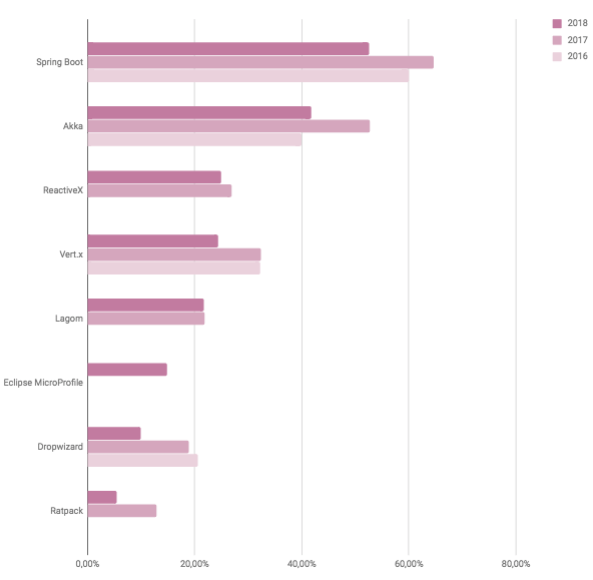
\includegraphics[width=.75\textwidth]{media/technologietrends.png}
	\label{jaxcenter:survey}
\end{figure}
\footnote{Schlosser und Richters, JAXenter-Survey: Application Frameworks - 2018, 2017, 2016 \cite{web:site:jaxcenter:trends}}
\end{center}

Gemäß den Technologietrends 2018 werden die Top 3 Spring-Boot, Akka und VertX betrachtet. Die korrespondierenden reaktiven Bibliotheken sind \hyperref[eval:rxjava]{\textbf{\nameref{eval:rxjava}}}, \hyperref[eval:reactor]{\textbf{\nameref{eval:reactor}}} und \hyperref[eval:akka-streams]{\textbf{\nameref{eval:akka-streams}}}. ReactiveX wird nicht als vollwertiges Framework wie Akka oder Spring betrachtet. Der Grund hierfür ist, dass ReactiveX sich selbst als API bezeichnet und nicht den technischen Umfang der anderen Frameworks aufweist. ReactiveX wird in vielen Programmiersprachen implementiert, weshalb die Verbreitung der ReactiveX API in Frontend (RxJs) und Backend (RxJava) stattfindet. Da Spring-Boot einen großen Umfang an Modulen besitzt, wird speziell das reaktive Web Framework WebFlux betrachtet.
\clearpage
Die folgende Abbildung zeigt einen Überblick über die bekanntesten reaktiven Frameworks/Toolkits und die dazugehörigen Bibliotheken.  

\begin{center}
\begin{figure}[H]
	\centering
    \caption{Überblick der reaktiven Bibliotheken und Frameworks}
    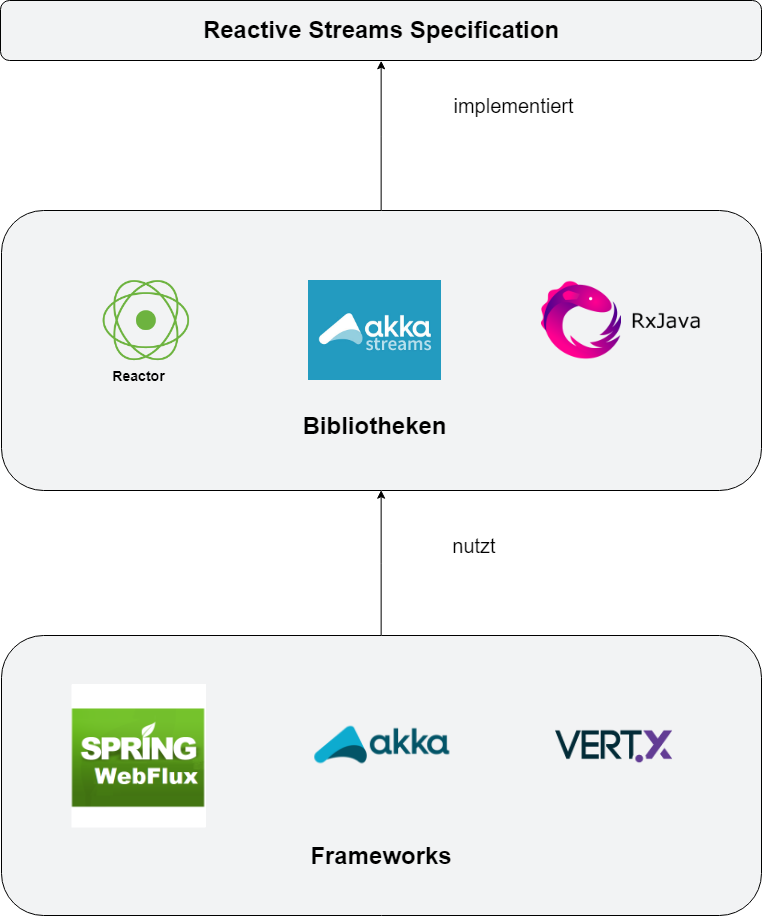
\includegraphics[width=.50\linewidth]{media/reactive_landscape}
    \label{benchmark}
\end{figure}
\end{center}

\section{Bibliotheken}
\subsection{Methodiken}
% Sonstige Befehle
\newcommand{\colorize}[1]{§\colorbox{yellow}{{#1}}§}
% Kriteriendefinition
\newcommand{\criteriaLizenz}{Lizenz und Kosten}
\newcommand{\criteriaSupport}{Support von Technologien}
\newcommand{\criteriaDoku}{Dokumentation}
\newcommand{\criteriaHandhabung}{Handhabung der Bibliothek}
\newcommand{\criteriaWeiterentwicklung}{Weiterentwicklung}
\newcommand{\criteriaVerbreitung}{Verbreitung}
Die Kriterien werden mittels der folgenden Methodiken evaluiert. Hierbei entsprechen die Kriterien den Anforderungen der Firma doubleSlash.

\begin{description}
\item \criteriaLizenz \\
Es ist zu prüfen ob die Bibliothek eine kommerzielle Nutzung zulässt und ob gegebenenfalls Kosten entstehen.
\item \criteriaDoku \\
Hierbei wird untersucht ob die Dokumentation umfassend, korrekt und aktuell ist.
\clearpage
\item \criteriaHandhabung \\
Es soll bewertet werden ob Programme kurz, prägnant und verständlich geschrieben werden können und ob eine falsche Bedienung verhindert bzw. erschwert wird.
\item \criteriaWeiterentwicklung \\
Es werden hierbei die Release-Daten untersucht und ermittelt ob Upgrades, Updates und Bugfixes regelmäßig erscheinen.
\item \criteriaVerbreitung \\
Die Ermittlung der Verbreitung wird zum einen über die Popularität auf GitHub verglichen und zum anderen über die Präsenz in der Entwickler-Community StackOverflow.
\end{description}

Die Bewertung der Kriterien beläuft sich auf ein Punkteschema. Jedes Kriterium wird zu Beginn mit zehn Punkten initialisiert. Für jedes negative Merkmal, dass bei der Betrachtung auffällt, gibt es Punktabzug. Die Menge an Punkten, die abzogen werden, richten sich nach der Schwere des Merkmals.

\subsection{RxJava}
\label{eval:rxjava}
RxJava steht für Reactive Extension (ReactiveX) Java. Die Reactive Extension wurde 2007 von Microsoft für .NET entwickelt. Die zunehmende Beliebtheit sorgte dafür, dass die API auch für andere Programmiersprachen implementiert wurde wie z. B. Javascipt, C\#, Scala, Swift, Clojure, C/C++, Python und viele mehr. Das Unternehmen Netflix hat RxJava implementiert und nutzt die Bibliothek für die Interprozesskommunikation und Verbindung verschiedener Services. In der Android Welt erfreut sich RxJava großer Beliebtheit. So nutzen Firmen wie SoundCloud, Square, NYT und Seatgeek die Bibliothek in ihren Apps.\footnote{vgl. Nurkiewicz und Christensen, Abs. 10 \cite{buch:reactive_programming_with_rxjava:foreword}}

RxJava gibt es in zwei Versionen. Version eins unterstützt nicht die Reactive Streams Specification und damit weder Back Pressure noch die Interkompatibilität mit anderen Bibliotheken. Version zwei dagegen ist eine Reimplementierung und unterstützt die Reactive Streams Specification. Im Rahmen dieser Thesis ist nur RxJava2 relevant. Die Bibliothek wird ab der Java Version 6 unterstützt.

Die Besonderheit von RxJava ist, dass die Daten der Publisher über Funktionen höherer Ordnung komponiert, gefiltert oder anderweitig transformiert werden können. Dieser funktionale Aspekt ermöglicht eine deklarative Programmierung. Unter dem Kriterium \href{handling:rxjava}{\criteriaHandhabung} wird gezeigt wie Nebenläufigkeit auf deklarative Art und Weise realisiert werden kann. 

Sowohl die Flow-Api als auch RxJava richten sich nach der Reactive Streams Specification. Folgende Tabelle zeigt die Flow-Typen und die RxJava Implementierungen: 

\begin{table}[H]
\centering
\caption{Flow Typen \& RxJava Typen (unvollständig)}
\begin{tabular}{|l|l|}
\hline
\rowcolor[HTML]{00A99D} 
Flow & RxJava \\ \hline
Publisher & Observable, Flowable \\ \hline
Subscriber & Observer, Single \\ \hline
Processor & Subject \\ \hline
Subscription & Disposable \\ \hline
\end{tabular}
\label{flow-api-to-rxjava}
\end{table}

Eine vollständige Liste der Typen in RxJava sind in der \href{http://reactivex.io/RxJava/javadoc/}{\textbf{Javadocs}} zu finden.

\subsubsection{\criteriaLizenz}
RxJava ist Open Source und besitzt die Apache-Lizenz 2.0 und ist daher für den kostenfreien, kommerziellen
Gebrauch zulässig. 

Da eine kommerzielle Nutzung erlaubt ist und keinerlei Kosten entstehen erhält RxJava zehn Punkte.

\begin{table}[H]
\begin{tabular}{|
>{\columncolor[HTML]{00A99D}}l |l|}
\hline
Punkte & 10 \\ \hline
\end{tabular}
\end{table}

\subsubsection{\criteriaDoku}
Auf der \href{https://reactivex.io}{\textbf{Homepage des Projekts}}\footnote{GitHub, ReactiveX Website \cite{web:site:reactivex}} befindet sich eine \href{http://reactivex.io/documentation}{\textbf{Referenzdokumentation}}, die die grundsätzlichen Typen und Mechanismen erklärt und illustriert. Diese Dokumentation soll primär die Kernkonzepte hinter ReactiveX vermitteln. Es handelt sich hierbei um eine allgemeine Referenz, die nicht programmiersprachenspezifisch ist.

Eine zweite Dokumentation gibt es auf GitHub in Form eines \href{https://github.com/ReactiveX/RxJava/wiki}{\textbf{Wiki}}\footnote{Github, ReactiveX Wiki \cite{web:github:reactivex:wiki}}. Das Wiki ist gut gegliedert und baut semantisch aufeinander auf. Für Java-Entwickler wird das Wiki für den Einstieg empfohlen, da alle relevanten Themen und weiterführende Informationen dort abgedeckt sind. Allerdings sind die Themen teils unvollständig dokumentiert.

Die \href{http://reactivex.io/RxJava/javadoc/}{\textbf{Javadocs}}\footnote{ReactiveX, Javadoc\cite{web:site:reactivex:javadoc}} lassen sich über das Wiki finden und sind auf dem aktuellen Stand des Releases. Die Dokumentation ist detailliert und enthält sämtliche Beschreibungen von Methoden, Klassen und Interfaces. Des Weiteren gibt es zu jeder Methode illustrierte Beispiele wie sie in der Praxis genutzt werden können.

Es gibt drei Punkte Abzug für die Unvollständigkeit der ReactiveX Referenzdokumentation. Die Überschriften im Wiki sind irreführend. Das Kapitel \href{https://github.com/ReactiveX/RxJava/wiki/Observable}{\textbf{reactive Types of RxJava}}\footnote{GitHub, ReactiveX Wiki \cite{web:github:reactivex:wiki:reactive_types}} suggeriert eine Auflistung der Typen, stattdessen wird auf die Referenzdokumentation verlinkt und der Observable Typ erklärt. 

\begin{table}[H]
\begin{tabular}{|
>{\columncolor[HTML]{00A99D}}l |l|}
\hline
Punkte & 7 \\ \hline
\end{tabular}
\end{table}

\subsubsection{\criteriaHandhabung}
\label{handling:rxjava}
Publisher und Subscriber können in RxJava kurz und prägnant ausgedrückt werden. Allerdings gibt es einige Aspekte, die eine falsche Benutzung ermöglichen. RxJava bietet eine Vielfalt an Typen für Publisher, Subscriber und Processor an. Das Problem ist, dass die große Menge an Typen eine umfangreichere Einarbeitung mit der Dokumentation benötigen. So wird in der Dokumentation als einziger reaktiver Typ das Observable genannt obwohl es weitaus mehr Typen für verschiedene Einsatzzwecke gibt. Das Flowable unterstützt Back Pressure während das Observable das nicht unterstützt. Die Verwechslung dieser Typen kann verheerend für das Programm sein.

Das folgende Listing zeigt ein Publisher (Flowable), welcher nacheinander die Events HELLO, WORLD und ! sendet. Der Subscriber (Observer) wird über zwei Methodenreferenzen und einer Lambda Funktion realisiert, welche implizit für die onNext, onError und onComplete Funktionen stehen. 

\begin{lstlisting}[language=java,  label={sourcecode:rxjava}, captionpos=t, caption={Synchron: RxJava Hello World}]
Flowable<String> flowable = Flowable.just("hello", "world", "!")
                                    .map(String::toUpperCase);
flowable.subscribe((next) -> 
				   System.out.println(Thread.currentThread.getName() 
				   						+ " " + next), // onNext
                   System.err::println,				   // onError
                   () -> System.out.println("done")); // onComplete
\end{lstlisting}
\clearpage

Das Programm erzeugt die folgende Ausgabe:

\begin{lstlisting}[language=bash,  label=ausgabe, captionpos=t, caption={Ausgabe vom synchronen Code}]
main HELLO
main WORLD
main !
done
\end{lstlisting}

Standardmäßig sind alle Publisher Typen (Observable, Flowable u. s. w.) synchron. Damit eine Subscription asynchron läuft, muss ein Threadpool respektiver Scheduler definiert werden, damit dieser auf einem Thread ausgelagert werden kann. Die Konfiguration hierfür ist allerdings simpel, da RxJava ein Set an Scheduler anbietet, die optimal auf das System abgestimmt sind. Das folgende Beispiel zeigt eine asynchrone Variante von \autoref{sourcecode:rxjava}.

\begin{lstlisting}[language=java,  label={sourcecode:rxjava:async}, captionpos=t, caption={Asynchron: RxJava Hello World (asynchron)}]
Scheduler scheduler = Schedulers.computation();
Disposable disposable = Flowable.just("hello", "world", "!")
.subscribeOn(scheduler) // Subscription auf einem Thread des Scheduler
.map(String::toUpperCase);
.subscribe(System.out::println,
     	   System.err::println,
           () -> System.out.println("done"));
while(!disposable.isDisposed()){}
\end{lstlisting}

Probleme in der Handhabung bei asynchroner Programmierung treten bei der Auswahl der Funktionen auf. RxJava bietet zwei Funktionen zur asynchronen Ausführung an. Zum einen subscribeOn (wie in \autoref{sourcecode:rxjava:async}) und zum anderen observeOn. Mit subscribeOn kann definiert werden mit welchem Scheduler die Subscription ausgelagert wird. Das heißt, dass alle Elemente auf einen anderen Thread geschickt werden und dort vom Subscriber über onNext, onError u. s. w. verarbeitet werden.

Die Funktion observeOn dagegen, definiert, auf welchen Thread einzelne Operationen ausgeführt werden können. Das heißt, dass alle Funktionen, die nach dem Aufruf von observeOn aufgerufen werden, auf einem anderen Thread laufen.

Das folgende Listing zeigt den Ausschnitt einer asynchronen Variante mit subscribeOn und observeOn. Über die Funktion doOnNext können schrittweise die Elemente ausgegeben werden. In diesem Beispiel wird der aktuelle Thread und das dazugehörige Element ausgegeben.
\clearpage
\begin{lstlisting}[language=java,  label={sourcecode:rxjava:async:debug}, captionpos=t, caption={RxJava Hello World debug}]
Flowable.just("hello", "world", "!")
.map(String::toUpperCase)
.doOnNext((element) -> System.out.println(Thread.currentThread()
										  .getName()+ " " + element))
.subscribeOn(scheduler)
.observeOn(scheduler) // Nachfolgende Funktionen auf anderem Thread des Schedulers
.filter(word -> word.length() > 1)
.subscribe((next) -> System.out.println(Thread.currentThread()
										      .getName()+" "+next),
                  System.err::println,
	              () -> System.out.println("done"));
\end{lstlisting}

Aufgrund dessen, dass das Programm multithreaded läuft, ist das nachfolgende Listing ein Beispiel:

\begin{lstlisting}[language=java,  label={sourcecode:rxjava:async:debug:ausgabe}, captionpos=t, caption={Ausgabe}]
RxComputationThreadPool-2 HELLO
RxComputationThreadPool-2 WORLD
RxComputationThreadPool-2 !
RxComputationThreadPool-1 HELLO
RxComputationThreadPool-1 WORLD
done
\end{lstlisting}

Die Ausgabe zeigt, dass die Verarbeitung des Flowables nicht auf dem Main Thread stattfindet, sondern auf dem RxComputationThreadPool-2 Thread. Die Funktionen, die nach dem Aufruf von observeOn folgen, werden auf dem RxComputationThreadPool-1 Thread ausgeführt wie z. B. der Aufruf der Filterfunktion. Das bedeutet, dass es entscheidend ist, wann die observeOn Funktion aufgerufen wird. Je nachdem wann die Funktion aufgerufen wird, werden alle folgenden Funktionen auf einem anderen Thread ausgelagert. Bei subscribeOn spielt die Reihenfolge keine Rolle, da die Subscription asynchron läuft und somit implizit der gesamte Stream mit allen Funktionen verlagert wird.

Bei der asynchronen Programmierung kann es schnell zur falschen Benutzung kommen, wenn die Anwendungsfälle der Funktionen nicht klar sind. Die freie Benutzung der Threadpools und Scheduler soll eine maximale Transparenz und eine freie Auswahl bezüglich Scheduler bieten. Für Anfänger wirkt das nicht intuitiv und verleitet zur falschen Benutzung.

Insgesamt gibt es zwei Punkte Abzug für die große Anzahl an Typen, die die API unübersichtlichen machen und eine falsche Benutzung der Typen ermöglichen. Des Weiteren gibt es noch zwei Punkte Abzug für das unkonventionelle Multithreading. Die deklarative Art erleichtert zwar die nebenläufige Programmierung, allerdings muss der Entwickler aufpassen in welchen Kontext, welche Funktion verwendet wird. Ein zu früh platzierter observeOn-Aufruf verlagert zu viele Operatoren auf einen anderen Thread und kann ihn überlasten. In der Praxis wird die observeOn-Funktion hinter der Subscribefunktion aufgerufen. Somit kann der Entwickler bestimmen, auf welchem Thread der Subscriber die Events verarbeitet. 
        
\begin{table}[H]
\begin{tabular}{|
>{\columncolor[HTML]{00A99D}}l |l|}
\hline
Punkte & 6 \\ \hline
\end{tabular}
\end{table}

\subsubsection{\criteriaWeiterentwicklung}
Um die Weiterentwicklung einer Bibliothek qualitativ zu bewerten werden Statistiken von dem Repository auf GitHub verglichen.

Der folgende Ausschnitt zeigt die Release-Zyklen des Projekts.
\begin{table}[H]
\caption{Ausschnitt aus den Releases}
\centering
\begin{tabular}{|l|l|}
\hline
\rowcolor[HTML]{00A99D} 
Version & Datum      \\ \hline
2.2.4   & 23.11.2018 \\ \hline
2.2.3   & 23.10.2018 \\ \hline
2.2.2   & 06.09.2018 \\ \hline
2.2.1   & 23.08.2018 \\ \hline
2.2.0   & 29.07.2018 \\ \hline
2.1.17  & 23.07.2018 \\ \hline
\end{tabular}
\end{table}

Es wird jeden Monat mindestens eine neue Version veröffentlicht. Die Nebenversionen werden hingegen unterschiedlich veröffentlicht. Die monatlichen Releases enthalten Bugfixes, Dokumentation und API-Erweiterungen. 

Insgesamt wird die Bibliothek aktiv weiterentwickelt und erhält regelmäßige Updates. Das Kriterium ist vollständig erfüllt.

\begin{table}[H]
\begin{tabular}{|
>{\columncolor[HTML]{00A99D}}l |l|}
\hline
Punkte & 10 \\ \hline
\end{tabular}
\end{table}

\subsubsection{\criteriaVerbreitung}
Um die Verbreitung einer Bibliothek zu messen werden verschiedene Metriken verwendet. Zum einen wird die Anzahl an getaggten Fragen auf StackOverflow verglichen. Die Anzahl sagt aus wie häufig Fragen bezüglich der Bibliothek gestellt werden. Die statistischen Werte auf GitHub sagen aus wie viele Personen sich für die Bibliothek interessieren. 

Die folgende Abbildung zeigt wie die Daten auf StackOverflow erhoben werden:
\begin{center}
\centering
\begin{figure}[H]
\caption{Erhebung der Daten auf StackOverflow}
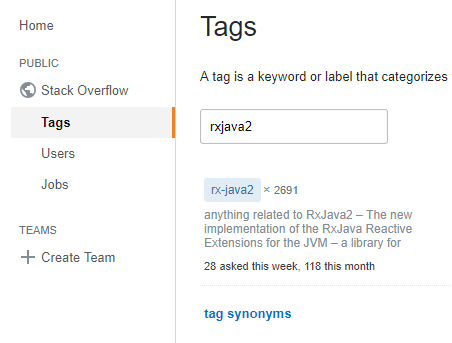
\includegraphics[width=.5\textwidth]{media/stackoverflow_rxjava}
\label{stackoverflow:rxjava}
\end{figure}
\end{center}

Die folgende Tabelle zeigt einen Schnappschuss aus StackOverflow\footnote{Quelle: \cite{web:site:stackoverflow:rxjava}, \cite{web:site:stackoverflow:akka}, \cite{web:site:stackoverflow:akka}}, wobei die Anzahl aktiv diskutierter Fragen im Kontext der jeweiligen Bibliothek betrachtet wird:

\begin{table}[H]
\centering
\caption{Schnappschuss aktiv diskutierter Fragen (Stand 03.12.2018)}
\begin{tabular}{|l|l|}
\hline
\rowcolor[HTML]{00A99D} 
Bibliothek   & Diskutierte Fragen \\ \hline
RxJava       & 2628   \\ \hline
Reactor     & 762    \\ \hline
Akka Streams & 1131   \\ \hline
\end{tabular}
\label{stackoverflow_snapshot}
\end{table}

Es zeigt sich, dass RxJava die am meisten diskutierte Bibliothek auf StackOverflow ist.

Die zweite Metrik stützt sich auf statistische Daten der Open Source Plattform GitHub. Hierbei wird die Anzahl an öffentlichen Repositories \footnote{Github Quelle zu den Repositories \cite{web:site:github:count:repo:rxjava} \cite{web:site:github:count:repo:reactor}, \cite{web:site:github:count:repo:akka}} sowie die Anzahl an Stars, die die Bibliothek hat, betrachtet. Die Stars eines Projektes sind als Wertschätzung für die Maintainer zu verstehen. GitHub nutzt diese Zahl zum globalen Ranking von Projekten.\footnote{vgl. GitHub, About Stars \cite{web:site:github:about_stars}} Damit wird die Popularität und Bekanntheit innerhalb der Community verstanden.

\begin{table}[H]
\caption{GitHub Statistik}
\centering
\begin{tabular}{l|l|l|l|}
\cline{2-4}
              & \cellcolor[HTML]{00A99D}RxJava & \cellcolor[HTML]{00A99D}Reactor & \cellcolor[HTML]{00A99D}Akka Stream \\ \hline
\multicolumn{1}{|l|}{\cellcolor[HTML]{00A99D}Repositories}  & 9005                          & 876                             & 836                                \\ \hline
\multicolumn{1}{|l|}{\cellcolor[HTML]{00A99D}Projekt Stars} & 36772                         & 2761                            & 9331                               \\ \hline
\multicolumn{1}{|l|}{\cellcolor[HTML]{00A99D}Ranking}		  & \href{https://gitstar-ranking.com/ReactiveX/RxJava}{48}							   & \href{https://gitstar-ranking.com/reactor/reactor}{3743}							 & \href{https://gitstar-ranking.com/akka/akka}{955}								   \\ \hline
\end{tabular}
\label{github:statistic}
\end{table}
\footnote{Da die Akka-Streams Bibliothek in Scala programmiert ist, wird die Anzahl Repositories unter der Sprache Scala betrachtet.}

Das Ranking wird über die Seite \href{www.gitstar-ranking.com}{www.gitstar-ranking.com}\footnote{Gitstar Quelle zum Ranking: \cite{web:site:gitstar-ranking:rxjava}, \cite{web:site:gitstar-ranking:reactor}, \cite{web:site:gitstar-ranking:akka}} ermittelt. 

Die Auswertung zeigt, dass RxJava mit über 8000 Repositories am häufigsten in Teilen von Projekten vorkommt. Des Weiteren hat die Bibliothek selbst über 36600 Stars, was unter den weltweiten Projekten (ca. 28 Millionen öffentliche Repositories)\footnote{Wikipedia \cite{web:wiki:github}} den 48. Platz belegt und somit weit vor Reactor und Akka steht.

Insgesamt ist RxJava auf StackOverflow die am meisten diskutierte Bibliothek. Auf GitHub werden statistisch mehr Projekte mit RxJava erstellt, das Repository der Bibliothek hat weitaus mehr Stars und belegt unter den Open Source Projekten den höchsten Platz. RxJava ist somit die am weitesten verbreitetste reaktive Bibliothek. Es gibt somit keinen Punktabzug.

\begin{table}[H]
\begin{tabular}{|
>{\columncolor[HTML]{00A99D}}l |l|}
\hline
Punkte & 10 \\ \hline
\end{tabular}
\end{table}

\subsection{Reactor}
\label{eval:reactor}
Die Bibliothek Reactor wird von Pivotal \& Spring vertrieben und implementiert die Reactive Streams Specification. Reactor wurde in Kollaboration mit Spring für das Webflux Framework entwickelt und ist ein Kernbestandteil davon. Aufgrund dessen das WebFlux relativ neu ist, unterstützt Reactor Java ab Version 8. Die folgende Tabelle zeigt eine Gegenüberstellung der Typen.

\begin{table}[H]
\caption{Flow \& Reactor (unvollständig)}
\centering
\begin{tabular}{|l|l|}
\hline
\rowcolor[HTML]{00A99D} 
Flow         & Reactor       \\ \hline
Publisher    & Flux, Mono    \\ \hline
Subscriber   & Subscriber    \\ \hline
Processor    & FluxProcessor \\ \hline
Subscription & Disposable    \\ \hline
\end{tabular}
\label{flow_to_reactor}
\end{table}

Weitere Typen und nähere Beschreibungen sind in der \href{https://projectreactor.io/docs/core/release/api/}{\textbf{Javadoc}}\footnote{Reactor, Javadoc \cite{web:site:reactor:javadoc} \label{lbl:reactor:javadoc}} zu finden.

\subsubsection{\criteriaLizenz}
Reactor ist Open Source und besitzt die Apache-Lizenz 2.0 und ist daher für den kostenfreien, kommerziellen
Gebrauch zulässig. 

Da eine kommerzielle Nutzung erlaubt ist und keinerlei Kosten entstehen, erhält Reactor keinen Abzug.
\begin{table}[H]
\begin{tabular}{|
>{\columncolor[HTML]{00A99D}}l |l|}
\hline
Punkte & 10 \\ \hline
\end{tabular}
\end{table}

\subsubsection{\criteriaDoku}
Reactor besitzt eine umfangreiche \href{https://projectreactor.io/docs/core/release/reference/}{Referenzdokumentation}\footnote{Reactor, Referenz \cite{web:site:reactor:reference}} und eine \href{https://projectreactor.io/docs/core/release/api/}{Javadoc}\footref{lbl:reactor:javadoc}. Die Referenz deckt grundlegende Fragen zur reaktiven Programmierung ab und führt in die Thematik ein. Des Weiteren wird auf die Installation, Kernkonzepte und weiter führende Themen eingegangen. Insgesamt ist die Referenz informativ und deckt alle Fragen für Neu- und Quereinsteiger ab.

Die Javadocs sind auf dem aktuellen Stand des Releases. Es werden in den Javadocs ebenfalls Illustrationen für die Funktionen verwendet.

Aufgrunddessen, dass Reactor eine geringe Anzahl an Typen hat, wirkt die API schlank und übersichtlich und ermöglicht schnelle Designentscheidungen im Bezug auf die Wahl der richtigen Typen.

Insgesamt ist die Referenzdokumentation als auch die Javadocs sehr übersichtlich und klar strukturiert. Die Reactor Bibliothek erhält die volle Punktzahl.

\begin{table}[H]
\begin{tabular}{|
>{\columncolor[HTML]{00A99D}}l |l|}
\hline
Punkte & 10 \\ \hline
\end{tabular}
\end{table}

\subsubsection{\criteriaHandhabung}
In Reactor können Publisher und Subscriber kurz und prägnant geschrieben werden. Die API ist der von RxJava sehr ähnlich. Der wesentliche Unterschied liegt darin, dass Reactor weniger Typen anbietet. Im Gegensatz zu RxJava bietet Reactor zwei Publisher-Typen an: Mono und Flux. Beide unterstützen standardmäßig das Back Pressure. Mono und Flux stehen jeweils für eine bestimmte Kardinalität. Mono verarbeitet Events in Anzahl 0 bis 1 während Flux 0 bis n verarbeitet. 

Das folgende Beispiel zeigt einen Flux, dass nacheinander HELLO, WORLD und ! emittiert.

\begin{lstlisting}[language=java, captionpos=t, caption={Synchron: Reactor Hello World!}, breaklines=true]
Flux<String> flux = Flux.just("hello", "world", "!")
                		.map(String::toUpperCase);
flux.subscribe((next)->System.out.println(Thread.getCurrentThread.getName()+" "+next),
               System.err::println,
               ()->System.out.println("done"));
\end{lstlisting}

Der Quellcode ist, bis auf die Namen, identisch mit dem Quellcode aus \ref{sourcecode:rxjava} in RxJava. 
Die Ausgabe ist äquivalent zur Ausgabe in \ref{ausgabe}. 

Bei der asynchronen Ausführung gibt es nur namentliche Unterschiede. Von der Menge des Codes und von der Semantik ist die Reactorimplementierung identisch mit der asynchronen Variante von RxJava in \ref{sourcecode:rxjava:async}. 
\clearpage
\begin{lstlisting}[language=java,  captionpos=t, caption={Asynchron: Reactor Hello World!}, breaklines=true]
Scheduler scheduler = Schedulers.parallel();
Disposable disposable = Flux.just("hello", "world", "!")
                            .map(String::toUpperCase)
                            .subscribeOn(scheduler)
                            .subscribe(
        	                    System.out::println,
                                System.err::println,
                                () -> System.out.println("done"));
while(!disposable.isDisposed()){}
\end{lstlisting}

Reactor hat, wie RxJava, ebenfalls zwei Methoden zur asynchronen Ausführung. Zum einen subscribeOn, welches dem subscribeOn in RxJava entspricht und zum anderen publishOn, was dem observeOn entspricht. Das Problem hierbei ist, wie bei RxJava, dass die Funktionen falsch benutzt werden können. \footnote{vgl. Kapitel \ref{handling:rxjava}} 

Zusammengefasst ist es relativ schwierig die Bibliothek falsch zu bedienen. Die schlanke API lässt es kaum zu, falsche Typen zu verwenden. Lediglich bei der asynchronen Programmierung können dieselben Probleme auftreten wie bei RxJava, weshalb die Bibliothek diesbezüglich zwei Punkte abgezogen bekommt.

\begin{table}[H]
\begin{tabular}{|
>{\columncolor[HTML]{00A99D}}l |l|}
\hline
Punkte & 8 \\ \hline
\end{tabular}
\end{table}

\subsubsection{\criteriaWeiterentwicklung}
Das Reactor Projekt wird in GitHub unter drei Versionen vertrieben. Version eins und zwei sind veraltet und werden nicht mehr aktiv weiterentwickelt. Für Version drei nutzen die Maintainer ein dreigleisiges Versionsschema. Die folgende Tabelle die Versionierung von Reactor3.

\begin{table}[H]
\caption{Versionsgleise und Versionsnummern}
\centering
\begin{tabular}{|l|l|}
\hline
\rowcolor[HTML]{00A99D} 
Versions-Gleis & Versionsnummer \\ \hline
Aluminium      & 3.0.x          \\ \hline
Bismuth        & 3.1.x          \\ \hline
Californium    & 3.2.x          \\ \hline
\end{tabular}
\end{table}

Die Versionsnummern entsprechen der Version der reactor-core Bibliothek. Die Reactor Bibliothek enthält zusätzlich zur Core Bibliothek noch einen Http und TCP Server (Reactor Netty) und Reactor Addons für die Interoperabilität zwischen verschiedenen Bibliotheken. Somit besteht die Reactor Bibliothek aus drei Unterbibliotheken.

Die Aluminium Version wurde seit zwei Jahren nicht mehr aktualisiert. Die Bismuth Version wird noch aktiv weiterentwickelt und erhält regelmäßig Updates. Die Hauptunterschiede zwischen den Nebenversionen sind Features und Namensänderungen. Die Versionsgleise sind somit nicht miteinander kompatibel.

\begin{table}[H]
\caption{Ausschnitt der Releases}
\centering
\begin{tabular}{|l|l|}
\hline
\rowcolor[HTML]{00A99D} 
Version & Datum      \\ \hline
3.2.3   & 23.11.2018 \\ \hline
3.2.2   & 31.10.2018 \\ \hline
3.2.1   & 10.10.2018 \\ \hline
3.2.0   & 21.09.2018 \\ \hline
3.1.0   & 25.09.2017 \\ \hline
3.0.0   & 23.08.2016 \\ \hline
\end{tabular}
\end{table}

Die Nebenversionen (Versionsgleise) werden kontinuierlich in Jahreszyklen veröffentlicht. Revisionen werden monatlich veröffentlicht.

Insgesamt wird die Bibliothek aktiv weiterentwickelt und erhält regelmäßig Updates. Das Kriterium ist vollständig erfüllt.

\begin{table}[H]
\begin{tabular}{|
>{\columncolor[HTML]{00A99D}}l |l|}
\hline
Punkte & 10 \\ \hline
\end{tabular}
\end{table}

\subsubsection{\criteriaVerbreitung}
\begin{table}[H]
\caption{GitHub Statistik}
\centering
\begin{tabular}{l|l|l|l|}
\cline{2-4}
              & \cellcolor[HTML]{00A99D}RxJava & \cellcolor[HTML]{00A99D}Reactor & \cellcolor[HTML]{00A99D}Akka Stream \\ \hline
\multicolumn{1}{|l|}{\cellcolor[HTML]{00A99D}Repositories}  & 9005                          & 876                             & 836                                \\ \hline
\multicolumn{1}{|l|}{\cellcolor[HTML]{00A99D}Projekt Stars} & 36772                         & 2761                            & 9331                               \\ \hline
\multicolumn{1}{|l|}{\cellcolor[HTML]{00A99D}Ranking}		  & \href{https://gitstar-ranking.com/ReactiveX/RxJava}{48}							   & \href{https://gitstar-ranking.com/reactor/reactor}{3743}							 & \href{https://gitstar-ranking.com/akka/akka}{955}								   \\ \hline
\end{tabular}
\label{github:statistic:reactor}
\end{table}

\begin{table}[H]
\centering
\caption{Schnappschuss aktiv diskutierter Fragen}
\begin{tabular}{|l|l|}
\hline
\rowcolor[HTML]{00A99D} 
Bibliothek   & Diskutierte Fragen \\ \hline
RxJava       & 2628   \\ \hline
Reactor     & 762    \\ \hline
Akka Streams & 1131   \\ \hline
\end{tabular}
\label{stackoverflow_snapshot:reactor}
\end{table}

Gemäß der Tabelle \ref{github:statistic:reactor} erreicht Reactor die niedrigste Platzierung der drei Bibliotheken. Auf StackOverflow erreicht Reactor ebenfalls eine geringere Anzahl an Fragen pro Tag, wie in \ref{stackoverflow_snapshot:reactor} zu sehen ist. Die Auswertung sagt nicht aus, dass die Bibliothek nicht verbreitet ist sondern, dass sie weniger verbreitet ist als Akka-Streams oder RxJava.

Da Reactor Kernbestandteil von Webflux ist, wird es implizit in allen Spring Webflux Anwendungen genutzt. Weiterhin bietet Spring zusätzlich eine Vielzahl an Integration an wie z. B. in Spring Data und Spring Security.

Allerdings ist Reactor eine Bibliothek, die stark an Popularität zunimmt. Der Chefentwickler von RxJava Dave Karnok antwortet auf die Frage, in welchen Situationen Reactor oder RxJava genutzt werden soll mit folgendem Satz: 
\begin{quote}
Use Reactor 3 if you are allowed to use Java 8+, use RxJava 2 if you are stuck on Java 6+ or need your functions to throw checked exceptions. \footnote{David Karnok, Twitter Posting \cite{web:site:twitter:feed:dave_karnok}}
\end{quote}

Insgesamt ist die Reactor Bibliothek, die am wenigsten verbreitete. Ausgehend von drei Plätzen, werden für jeden Platz 3 Punkte vergeben. Der Erste erhält 4 Punkte dem zweiten gegenüber. Somit bekommt die Bibliothek 7 Punkte Abzug.

\begin{table}[H]
\begin{tabular}{|
>{\columncolor[HTML]{00A99D}}l |l|}
\hline
Punkte & 3 \\ \hline
\end{tabular}
\end{table}

\subsection{Akka-Streams}
\label{eval:akka-streams}
\label{intro:akka-streams}
Akka-Streams ist die Stream Bibliothek des Akka Toolkits und wird ab der Javaversion 8 unterstützt. Die Besonderheit der Bibliothek ist, dass die Flow Typen nicht direkt als Schnittstelle angeboten werden sondern ausschließlich über die Implementierungen zur Verfügung stehen. Das heißt, dass die Publisher, Subscriber u. s. w. nicht direkt zugänglich sind. Die Entwickler der Akka-Streams betrachten die Reactive Streams Specification nicht als End-User API sondern als SPI (Service Provider Interface). \footnote{vgl. Lightbend, Inc., Relationship with Reactive Streams, 2018 \cite{web:akka:def:streams}} Das heißt, dass die Schnittstelle ausschließlich für die Entwickler freigegeben wird und nicht für die Nutzer der Bibliothek. Die schwer zu implementierenden Interfaces sollen somit verborgen bleiben und über einfachere Abstraktionen bedienbar sein. Bibliotheken wie RxJava und Reactor bieten auch Abstraktionen zu Publishern und Subscriber an (Observable, Flux), allerdings kann der Entwickler auch eigene Publisher implementieren.

Die folgende Tabelle stellt die Flow Typen den Akka-Streams Typen gegenüber: 

\begin{table}[H]
\caption{Flow \& Akka-Streams}
\centering
\begin{tabular}{|l|l|}
\hline
\rowcolor[HTML]{00A99D} 
Flow         & Akka-Streams \\ \hline
Publisher    & Source       \\ \hline
Subscriber   & Sink         \\ \hline
Processor    & Flow         \\ \hline
Subscription & Materializer \\ \hline
\end{tabular}
\label{flow_to_akka}
\end{table}
\clearpage
Ein Typischer Akka Stream sieht wie folgt aus:

\begin{center}
\begin{figure}[H]
\centering
\caption{Akka-Stream Beispiel}
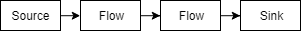
\includegraphics[width=.75\textwidth]{media/akka-stream}
\label{fig:akka-stream}
\end{figure}
\end{center}

Eine oder mehrere Sources definieren die Datenquelle und können Nachrichten aus primitiven Datentypen, Collections und Arrays erzeugen. Am Ende der Verarbeitungskette befinden sich eine oder mehrere Sinks, welche die ankommenden Daten verarbeiten. Zwischen Source und Sink können Flows platziert werden, die weitere Verarbeitungsschritte umsetzen. Der Materializer alloziert die notwendigen Ressourcen der Prozessschritte und führt diese aus. Diese Art der Verarbeitung ermöglicht eine Entkoppelung der Verarbeitungsschritte und damit eine Wiederverwendung. \footnote{vgl. Lightbend Inc., Core Concepts \cite{web:akka:docs:streams_flows_and_basics}\label{akka:concept}}

In Akka-Streams werden Verarbeitungsketten von Source, Flows und Sinks als Graphen bezeichnet. Ein Graph beschreibt die Topologie der Verarbeitungsschritte. Der Stream aus \autoref{fig:akka-stream} ist ein trivialer Graph. Komplexe Graphen können auch aus mehreren Eingabe- und Ausgabekanälen bestehen. 

\subsubsection{\criteriaLizenz}
Akka-Stream ist Open Source und besitzt die Apache-Lizenz 2.0 und ist daher für den kostenfreien, kommerziellen
Gebrauch zulässig.

Da eine kommerzielle Nutzung erlaubt ist und keinerlei Kosten entstehen erhält Akka-Stream 10 Punkte.
\begin{table}[H]
\begin{tabular}{|
>{\columncolor[HTML]{00A99D}}l |l|}
\hline
Punkte & 10 \\ \hline
\end{tabular}
\end{table}

\subsubsection{\criteriaDoku}
Akka bietet eine übersichtliche \href{https://akka.io/docs/}{\textbf{Referenzdokumentation}}\footnote{Lightbend, Docs \cite{web:akka:docs}} für alle Module an. Hierbei können Code-Beispiele wahlweise in Scala oder Java betrachtet werden. Module, die Teil von Akka sind, entsprechen immer der Repository Version. Die aktuelle Akka Version ist 2.5.19 (Stand 10.12.2018). Die \href{https://doc.akka.io/docs/akka/current/stream/index.html?language=java}{\textbf{Akka-Stream Referenz}}\footnote{Lightbend, Referenz \cite{web:akka:docs:streams}} bietet eine gegliederte Übersicht über alle Teilaspekte der Streams an wie z. B. grundlegende Datentypen wie Source und Sink, IO Verarbeitung, Graphen u. v. m. .

Die \href{https://doc.akka.io/japi/akka/current/index.html?akka/stream/package-summary.html&_ga=2.134194124.394401883.1544449904-1435486093.1536821504}{\textbf{Javadocs}}\footnote{Lightbend, Javadoc \cite{web:akka:javadoc}} sind auf dem aktuellen Stand des Releases. Ein Problem der Dokumentation ist, dass sie nicht nur die Streams enthält, sondern alle restlichen Akka Module wie z. B. Actor, Cluster und Persistence. Das hat zur Folge, dass die Doku sehr umfangreich und unübersichtlich ist. Die Beschreibung ist detailliert und teilweise mit Code-Beispielen versehen.

Insgesamt sind die Javadocs gut und hilfreich, allerdings werden einige Funktionen wie z. B. fold und scan rein textuell erklärt und weder mit Code-Beispielen noch mit Diagrammen vereinfacht dargestellt. Hierfür gibt es 2 Punkte Abzug. Die folgende Abbildung zeigt ein Beispiel der schlecht dokumentierten Funktion scan und fold:

\begin{center}
\begin{figure}[H]
\centering
\caption{Ausschnitt aus der Dokumentation der Funktionen scan und fold}
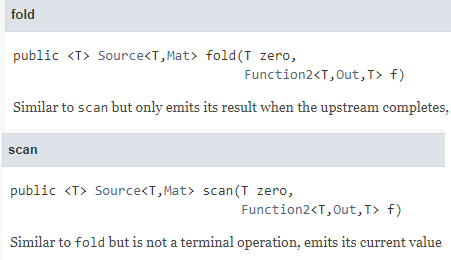
\includegraphics[width=.75\textwidth]{media/genius}
\label{fig:akka-stream:javadoc}
\end{figure}
\end{center}

Die Referenzdokumentation hat relativ schwer nachvollziehbare Codebeispiele, die das Wesentliche kompliziert darstellen. Hierfür gibt es drei Punkte Abzug, da für das Kapitel \href{https://doc.akka.io/docs/akka/current/stream/stream-graphs.html}{Working with Graphs} einiges an Recherche gemacht werden muss, die nicht in den Grundlagen erklärt werden.

\begin{table}[H]
\begin{tabular}{|
>{\columncolor[HTML]{00A99D}}l |l|}
\hline
Punkte & 5 \\ \hline
\end{tabular}
\end{table}

\subsubsection{\criteriaHandhabung}
Publisher und Subscriber können bedingt kurz und prägnant ausgedrückt werden. Grundsätzlich unterscheidet sich die Akka-Stream Bibliothek sehr stark von RxJava und Reactor. Das Vokabular rund um Akka-Stream ist deutlich größer als das von RxJava oder Reactor. Der Code sieht unübersichtlich aus und enthält viele Typen. Allerdings entfällt die Unübersichtlichkeit und der Boilerplate Code, wenn Scala statt Java verwendet wird. Akka-Stream ist eine Bibliothek, die in erster Linie in Scala entwickelt wurde und die Eigenschaften dieser Sprache optimal nutzt. In Java wirkt der Code deutlich komplexer, was auch die Handhabung beeinträchtigt.

Das folgende Beispiel demonstriert das (asynchrone) Emittieren von HELLO, WORLD und !.

\begin{lstlisting}[language=java,  label={sourcecode:akka}, captionpos=t, caption={Akka Streams Hello World}, breaklines=false]
ActorSystem actorsystem = ActorSystem.create();
Materializer materializer = ActorMaterializer.create(system);
Source<String, NotUsed> source = Source
								 .from(Arrays.asList("hello",
								 					 "world",
								 					 "!"))
                                 .map(String::toUpperCase);
Sink<String, CompletionStage<Done>> sink = Sink
										   .foreach(System.out::println);
CompletionStage<Done> done = source.runWith(sink, materializer);
done.thenRun(() -> {
	System.out.println("done");
    actorsystem.terminate();});
\end{lstlisting}

Die Ausgabe ist äquivalent zur Ausgabe in \autoref{ausgabe}.

In Akka erfolgt die Kommunikation zwischen asynchronen Endpunkten immer über Nachrichten mehrerer Aktoren. Damit ein Programm die Aktoren nutzen kann, benötigt es eine Laufzeitumgebung für die Aktoren, dem Aktorensystem (Zeile 1). Wie in \autoref{intro:akka-streams} bereits beschrieben, werden Definition und Ausführung getrennt. In Zeile 2 wird der Materializer aus dem Aktorensystem erzeugt. Der Materializer alloziert die Ressourcen für die Verarbeitungsschritte und führt diese aus. Die Verarbeitungsschritte entsprechen in  in Listing \ref{sourcecode:akka} Source (Zeile 3) und Sink (Zeile 8). Über die Methode runWith wird die Source mit dem Sink verknüpft und über den Materializer ausgeführt. Da standardmäßig die Streams asynchron ausgeführt werden, muss das Aktorensystem terminiert werden, sobald das Programmende erreicht wurde. Der erste generische Typ der Source gibt den Typen des Ausgabeparameters an. Der zweite gibt Hilfsinformationen an, wie z. B. Netzwerkinformationen Ports, IP-Adressen und ähnliches. In Anwendungen in denen keine Hilfsinformationen genutzt werden, wird der Typ NotUsed verwendet. \footnote{vgl. Lightbend Inc., Streams Quickstart Guide \cite{web:akka:docs:stream_quickstart_guide}} Im Sink entspricht der erste Typ dem Eingabeparameter und der zweite dem Eingabeparameter für Hilfsinformationen. Das \href{https://docs.oracle.com/javase/8/docs/api/java/util/concurrent/CompletionStage.html}{\textbf{CompletionStage}} ist ein Typ für asynchrone Verarbeitung aus dem java.util.concurrent Package.

Die Handhabung der Akka-Streams Bibliothek ist unkompliziert. Der Java-Code hat einiges an Boilerplate Code und viele generische Typen, dass zum einen die Lesbarkeit erschwert und zum anderen komplexer wirkt im Vergleich zu anderen Bibliotheken wie RxJava und Reactor. Eine falsche Bedienung ist schwer zu bewerkstelligen. Zwar wird das Aktorensystem und der Materializer benötigt, allerdings sind diese Pflichtbestandteil eines jeden Akka-Streams-Programm. Aufgrund dessen, dass Java die Programmiersprache in der Betrachtung ist, erhält Akka-Streams vier Punkte Abzug in der Handhabung. 

\begin{table}[H]
\begin{tabular}{|
>{\columncolor[HTML]{00A99D}}l |l|}
\hline
Punkte & 6 \\ \hline
\end{tabular}
\end{table}

\subsubsection{\criteriaWeiterentwicklung}
Da es kein gesondertes Repository für die Akka-Stream Bibliothek gibt, werden zur Evaluierung die Repositories Alpakka und Akka betrachtet. Alpakka ist eine ergänzende Bibliothek und stellt Adapter Klassen für verschiedene Technologien bereit um mit Akka-Streams zu arbeiten. Somit lässt sich Alpakka mit den Reactor Addons vergleichen. Es gibt noch ein Contributer Repository für Akka-Streams. Allerdings ist dieser primär als Erweiterung für die Akka-Streams API gedacht und ist nicht Teil der Core Bibliothek. 

Die folgende Tabelle zeigt einen Auszug aus den Realeases von Akka und Alpakka.

\begin{table}[H]
\centering
\caption{Auszug aus den Releases von Akka und Alpakka}
\label{tbl:release:akka-alpakka}
\begin{tabular}{|l|l|l|l|}
\hline
\rowcolor[HTML]{00A99D} 
\multicolumn{2}{|l|}{\cellcolor[HTML]{00A99D}{\color[HTML]{FFFFFF} Akka}} & \multicolumn{2}{l|}{\cellcolor[HTML]{00A99D}{\color[HTML]{FFFFFF} Alpakka}} \\ \hline
\rowcolor[HTML]{00A99D} 
{\color[HTML]{FFFFFF} Version} & {\color[HTML]{FFFFFF} Datum} & {\color[HTML]{FFFFFF} Version} & {\color[HTML]{FFFFFF} Datum} \\ \hline
2.5.19 & 07.12.2018 & 1.0.0 & 06.11.2018 \\ \hline
2.5.18 & 07.11.2018 & 0.2.0 & 04.07.2018 \\ \hline
2.5.17 & 27.09.2018 & 0.19.0 & 09.05.2018 \\ \hline
2.0.0 & 06.03.2012 & 0.18.0 & 28.03.2018 \\ \hline
1.0.0 & 15.02.2011 & 0.17.9 & 19.2.2018 \\ \hline
\end{tabular}
\end{table}


Bei Akka werden Revisionen monatlich aktualisiert. Hauptversionen werden in unregelmäßigen Zeitabständen veröffentlicht. So liegt zwischen Version 1.0 und 2.0 ca. ein Jahr, während zwischen 2.0 und 2.5 ca. fünf Jahre liegen. Nebenversionen werden ebenfalls unterschiedlich veröffentlicht. 

Im Akka Repository werden mithilfe von Labels die jeweiligen Module gekennzeichnet, um Issues und Commits zu referenzieren. Die Akka-Stream Bibliothek wird unter dem Label \href{https://github.com/akka/akka/labels/t\%3Astream}{t:stream} weiterentwickelt. 

Die Alpakka Bibliothek erhielt alle ein bis zwei Monate ein Update auf die nächste Nebenversion. Version 1.0 ist der aktuelle Release (Stand 10.12.2018). 

Es lässt sich sagen, dass Akka-Streams (Akka) und Alpakka weiterentwickelt werden. Die Updatezyklen der Haupt- und Nebenversionen sind relativ ungenau zu bestimmen, jedoch kommen regelmäßige Updates und Bugfixes (siehe Revisionen in \autoref{tbl:release:akka-alpakka}). Somit bekommt die Bibliothek 10 Punkte.

\begin{table}[H]
\begin{tabular}{|
>{\columncolor[HTML]{00A99D}}l |l|}
\hline
Punkte & 10 \\ \hline
\end{tabular}
\end{table}

\subsubsection{\criteriaVerbreitung}
\begin{table}[H]
\caption{GitHub Statistik}
\centering
\begin{tabular}{l|l|l|l|}
\cline{2-4}
              & \cellcolor[HTML]{00A99D}RxJava & \cellcolor[HTML]{00A99D}Reactor & \cellcolor[HTML]{00A99D}Akka Stream \\ \hline
\multicolumn{1}{|l|}{\cellcolor[HTML]{00A99D}Repositories}  & 9005                          & 876                             & 836                                \\ \hline
\multicolumn{1}{|l|}{\cellcolor[HTML]{00A99D}Projekt Stars} & 36772                         & 2761                            & 9331                               \\ \hline
\multicolumn{1}{|l|}{\cellcolor[HTML]{00A99D}Ranking}		  & \href{https://gitstar-ranking.com/ReactiveX/RxJava}{48}							   & \href{https://gitstar-ranking.com/reactor/reactor}{3743}							 & \href{https://gitstar-ranking.com/akka/akka}{955}								   \\ \hline
\end{tabular}
\label{github:statistic:akka}
\end{table}

\begin{table}[H]
\centering
\caption{Schnappschuss aktiv diskutierter Fragen}
\begin{tabular}{|l|l|}
\hline
\rowcolor[HTML]{00A99D} 
Bibliothek   & Diskutierte Fragen \\ \hline
RxJava       & 2628   \\ \hline
Reactor     & 762    \\ \hline
Akka Streams & 1131   \\ \hline
\end{tabular}
\label{stackoverflow_snapshot:akka}
\end{table}

Gemäß der \autoref{github:statistic:akka} belegt Akka den 2. Platz. Die Wertung bezieht sich allerdings auf das Akka Repository und nicht auf die Akka-Stream Bibliothek. Das liegt daran, dass die Akka-Stream Bibliothek ein Teil von dem Akka Repository ist.

Auf StackOverflow (siehe \autoref{stackoverflow_snapshot:akka}) werden Akka-Streams am zweithäufigsten diskutiert. Aufgrund dessen, dass auf StackOverflow gezielt nach Tags gesucht werden kann, wird hier nach Akka-Stream gesucht.

Zusammengefasst belegt Akka-Stream den zweiten Platz unter den drei evaluierten Bibliotheken. Somit werden der Akka-Stream Bibliothek 4 Punkte abgezogen. 

\begin{table}[H]
\begin{tabular}{|
>{\columncolor[HTML]{00A99D}}l |l|}
\hline
Punkte & 6 \\ \hline
\end{tabular}
\end{table}

\section{Bewertung}
\label{sec:bewertung}
Die Auswertung erfolgt mittels einer gewichteten Evaluationsmatrix. Die Kriterien und die Gewichtung entsprechen den Vorgaben des Unternehmens doubleSlash.

\begin{table}[H]
\caption{Gewichtete Evaluationsmatrix}
\centering
\resizebox{\textwidth}{!}{%
\begin{tabular}{|l|c|c|c|c|c|c|c|}
\hline
 & \multicolumn{1}{l|}{} & \multicolumn{2}{c|}{RxJava} & \multicolumn{2}{c|}{Project Reactor} & \multicolumn{2}{c|}{Akka-Streams} \\ \hline
Kriterium & Gewichtung & Punkte & gew. Punkte & Punkte & gew. Punkte & Punkte & gew. Punkte \\ \hline
Lizenz in Geschäftsanwendungen & 3 & 10 & 30 & 10 & 30 & 10 & 30 \\ \hline
Dokumentation & 3 & 7 & 21 & 10 & 30 & 5 & 15 \\ \hline
Handhabung der Bibliothek & 2 & 6 & 12 & 8 & 16 & 6 & 12 \\ \hline
Weiterentwicklung & 1 & 10 & 10 & 10 & 10 & 10 & 10 \\ \hline
Verbreitung & 1 & 10 & 10 & 3 & 3 & 6 & 6 \\ \hline
Ergebnis &  &  & 83 &  & 89 &  & 73 \\ \hline
\end{tabular}%
}
\label{matrix}
\end{table}

Die Evaluationsmatrix zeigt, dass Reactor knapp vor RxJava und weit vor Akka-Streams liegt. Das liegt daran, dass Reactor eine bessere Dokumentation und eine bessere Handhabung aufweist. Für die Konzeption der prototypischen Anwendung wird daher die Reactor Bibliothek verwendet.

\section{Frameworks}
\label{section:frameworks}
\subsection{Spring Webflux}
Mit Version 5 des Spring Frameworks, wurde das WebFlux Modul eingeführt, dass eine nicht-blockierende, reaktive Alternative zum klassischen Spring-MVC Modul ist. Kernbestandteil von Webflux ist die Reactor Bibliothek, welche eine Implementierung für Reactive Streams ist. Die folgende Abbildung zeigt das Spring 5 Framework mit den neu hinzugekommenen Modulen (grün markiert). \footnote{vgl. Reddy, Reactive Web Applications Using Spring WebFlux \cite{buch:beginning_spring_boot2:kapitel12} \label{webflux:book}}

\begin{center}
\begin{figure}[H]
    \caption{Spring 5 Module}
    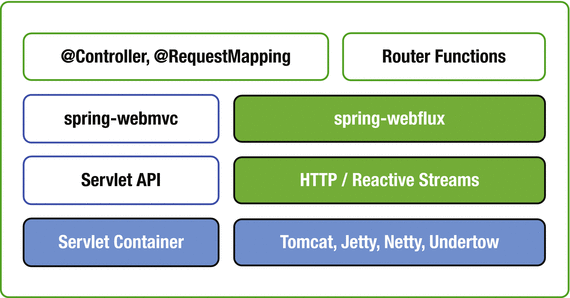
\includegraphics[width=\linewidth]{media/Spring5-runtime}
	\footref{webflux:book}    
    \label{spring5-runtime}
\end{figure}
\end{center}

WebFlux läuft grundsätzlich auf asynchronen Laufzeitumgebungen wie Tomcat, Jetty, Undertow und Netty. Es werden nur Servlet Container unterstützt, die mindestens die Servlet-Spezifikation V. 3.1 implementieren. \footref{webflux:book}

\subsection{Akka}
Akka ist ein Toolkit, daher eine Sammlung von Bibliotheken, mit dem sich Reactive Systeme realisieren lassen. Das heißt, dass Technologien die entsprechend dem  \autoref{sec:das_reaktive_manfiest} notwendig sind, bereits im Repertoire von Akka sind. Die folgende Tabelle fasst einige Akka Module zusammen.

\begin{table}[H]
\caption{Unvollständige Liste der Akka Module}
\centering
\begin{tabular}{|l|l|}
\hline
\rowcolor[HTML]{00A99D} 
{\color[HTML]{FFFFFF} Akka Modul}      & {\color[HTML]{FFFFFF} Beschreibung}                                                                                                              \\ \hline
Actors           & \begin{tabular}[c]{@{}l@{}}Implementierung des Aktorenmodells\\ zur nachrichtenbasierten Kommunikation\end{tabular}       \\ \hline
Streams          & \begin{tabular}[c]{@{}l@{}}Für nicht-blockierende und nebenläufige \\ Verarbeitung von Daten\end{tabular}                 \\ \hline
Cluster          & \begin{tabular}[c]{@{}l@{}}Ermöglich Skalierung und Widerstandsfähigkeit\\ durch Verteilung auf mehreren Knoten\end{tabular} \\ \hline
Distributed Data & \begin{tabular}[c]{@{}l@{}}Ermöglicht einen Lese- und Schreibzugriffe \\ mit geringer Latenzzeit auf Knoten.\end{tabular}    \\ \hline
\end{tabular}
\end{table}
\footnote{vgl. Akka Docs, \cite{web:akka:docs}}

Auf der Anwendungsebene nutzt Akka die Akka-Streams als Reactive Streams Implementierung. Prominente Unternehmen, die Akka aktiv in ihrem Production Code nutzen sind unter anderem Paypal, Twitter, Samsung, Intel, Verizon und LinkedIn. 

\subsection{Eclipse Vert.x}
Vert.X (ausgeprochen Vertex) ist ein Toolkit für nebenläufige und nicht-blockierende Anwendungen für die JVM. Das Toolkit basiert auf dem Netty Project und bietet eine High-Level API für das zugrunde liegende Netty Framework. Weiterhin ist Vert.X mehrsprachig, also ein Toolkit, dass mehrere Sprachen unterstützt, die auf der JVM laufen. Somit gibt es Support für Java, Scala, Kotlin, Groovy, Javascript, Ruby und Ceylon. \footnote{vgl. Ponge, Segismont \& Viet et al. , Seite 2-6, \cite{buch:a_gentle_guide:kapitel1} \label{vertx:intro}}

Konzeptuell hat Vert.X zwei Kernaspekte. Zum einen das Verticle und zum anderen den Eventbus. Ein Verticle ist eine Verarbeitungseinheit. Es beinhaltet eine Eventloop, in der Events entgegengenommen werden. Per Default werden zwei Verticle pro CPU Kern zur Verfügung gestellt. Der Eventbus ist für die asynchrone Kommunikation zwischen den Verticles zuständig. Zwischen Verticles wird über Nachrichten kommuniziert. Ähnlich zu Akka kann mit dem Vert.X Toolkit reaktive Systeme gebaut werden. \footref{vertx:intro}

Vert.X bietet zwei Arten von Reactive Streams an. Zum einen die Reactive Streams Integration für die Read/Write Streams, wobei es sich es um eine Überbrückung von Read/Write Stream zu Publisher/Subscriber handelt. \footnote{vgl. tsegismont, StackOverflow Kommentar \cite{web:site:stackoverflow:vertx:comment}} Zum Anderen die RxJava- Streams, allerdings wurde die Bibliothek entsprechend dem Toolkit angepasst. Das heißt es wurden einige Funktionen entfernt, die nicht mit den Modulen aus Vert.X arbeiten können. Umgekehrt wurde auch die Vert.X API an RxJava angepasst, der sogenannten Rxified API.

Bekannte Unternehmen wie Bosch, VmWare, Hulu, Zalando, Deutsche Börse Group, Red Hat und viele andere nutzen Vert.X in ihren Projekten. \footnote{vgl. Vert.X Homepage, \cite{web:site:vertx}}